\chapter{Monte Carlo Simulation}
\label{cap:montecarlo}

The modern version of the Monte Carlo method dates back to the introduction of the first computers and their application during the years 1940-45 with the purpose of computing neutron diffusion in atomic bombs.

The Monte Carlo approach was primarily promoted by physics researchers Stanislaw Ulam, Nicholas Metropolis and John von Neumann.

They were well aware of the potential of such techniques but it was only with the first electronic computer, the ENIAC, which was able to solve differential equations at a tremendous so far inconceivable speed, the Monte Carlo method was eventually triggered.

The name Monte Carlo refers to a famous casino in Monaco where Ulam's uncle used to indulge his gambling passion. 
The characteristics of randomness and the repetitive nature of many processes correspond with the games played in a casino. Note that the famous roulette wheel is one of the simplest mechanical devices to generate random variables.

Simulation tools find their application mostly in cases where the inherent complexity of a problem makes the use of other techniques impossible or where no analytically tractable solution with a
deterministic algorithm is existing. In short, \emph{the Monte Carlo method is a numerical approach which aims for solving mathematical problems by the simulation of random variables}.

Monte Carlo simulations are widely used in many fields: Engineering, Physics, Computational biology, Computer graphics, Applied statistics and Artificial intelligence for games.

It started to be en vogue in financial mathematics in the 1980s, particularly when the theories of the random walk of asset prices came up.

%The modern version of the Monte Carlo method was invented in the late
%1940s by Stanislaw Ulam, while he was working on nuclear weapon
%projects at the Los Alamos National Laboratory.

%Monte Carlo methods, or experiments, are a broad class of computational
%algorithms that rely on repeated random sampling to obtain numerical
%results; the underlying concept is to use randomness to solve problems
%that might be deterministic in principle. Monte Carlo methods are mainly
%used in three problem classes: optimization, numerical integration, and
%generating draws from a probability distribution.

In this Chapter this very important technique is reviewed and presented beside some applications.

\section{The Algorithm}
\label{whats-monte-carlo-simulation}

Monte Carlo (MC) methods are used when a closed-form solution for a property being studied cannot be developed (i.e. the probability of varying outcomes cannot be determined because of random variable interference).

When faced with significant uncertainty in the process of making a forecast or estimate, rather than just replacing the uncertain variable with a single average number, the Monte Carlo Simulation might prove to be a better solution by using multiple values.
This is achieved by building models of possible results where any factor that has inherent uncertainty (random variables) is replaced with a range of values (i.e. a probability distribution).

A Monte Carlo simulation takes the variables that have uncertainty and assigns them a random value. The model is then run and a result is provided. This process is repeated again and again while assigning the variables in question with many different values. Once the simulation is completed, the results are averaged together to provide an estimate or the distribution of possible outcome values is drawn.

Note that depending upon the number of uncertainties and the ranges specified for them, a Monte Carlo simulation could involve thousands or tens of thousands of recalculations before it is completed.

A MC method/algorithm then can be described as follows:

\begin{itemize}
\item  identify the independent and dependent variables and define their domain $\Omega$ of possible inputs (probability distributions for our inputs);
\item generate random inputs from the domain \(\Omega\);
\item compute the model output based on the randomly generated inputs;
\item repeat the experiment N number of times and aggregate the results.
\end{itemize}

Imagine to simulate the results of rolling a die: the only variable is the die outcome,  $\Omega =1,2,3,4,5,6$, the outcome probability is a uniform distribution since every result is equiprobable. So the simulation consists of sampling uniform distributed integers between 1 and 6.

In the next Sections we will see each step in the implementation of practical examples.

\section{Pseudo-Random Numbers}
\label{pseudo-random-numbers}

The need of generating random inputs during a MC simulation requires large amounts of \emph{random numbers} to be generated, and it was their use that spurred the development of pseudo-random number generators. 

Nowadays every programming language has libraries that allows to produce huge series of random numbers. These series, which have very large periodicity (e.g. \(2^{19937}\)), are calculated by algorithms that take as input a \emph{seed} which determines them uniquely. This means that choosing the same seed you will produce the same set of numbers every time (which is great for debugging purposes).

In \texttt{python} one of the available modules to generate random numbers is \texttt{random} which has, among others, the following useful functions:
\begin{itemize}
\tightlist
\item
  \texttt{seed}: set the seed of the random number generator;
\item
  \texttt{random}: returns a random number between 0 and 1 (with uniform
  probability);
\item
  \texttt{randint(min,\ max)}: returns an integer random number between
  \texttt{min} and \texttt{max} (with uniform probability);
\item
  \texttt{sample(aList,\ k=n)}: samples n elements from the list
  \texttt{aList}.
\end{itemize}
\noindent
For a more detailed description check \texttt{help(random)}.

The following example shows an application of these functions beside the effect of  changing the random number generator seed.

\begin{ipython}
import random

random.seed(1)
print ("seed is 1")
print(random.random())
print(random.random())
\end{ipython}
\begin{ioutput}
seed is 1
0.13436424411240122
0.8474337369372327
\end{ioutput}
\begin{ipython}
random.seed(2)
print ("seed is 2")
print(random.random())
print(random.random())
\end{ipython}
\begin{ioutput}
seed is 2
0.9560342718892494
0.9478274870593494
\end{ioutput}
\begin{ipython}
random.seed(1)
print ("seed is 1 again")
print(random.random())
print(random.random())
\end{ipython}
\begin{ioutput}
seed is 1 again
0.13436424411240122
0.8474337369372327
\end{ioutput}
\begin{ipython}
print(random.randint(1, 10))
aList = ['a', 'b', 'c', 'd', 'f']
print (random.sample(aList, k=2))
\end{ipython}
\begin{ioutput}
2
['c', 'a']
\end{ioutput}

The next lines of code show instead how to draw a uniform distribution. Figure~\ref{fig:uniform_dist} reports the result.

\begin{ipython}
from matplotlib import pyplot as plt

numbers = []
for _ in range(10000):
    numbers.append(random.randint(0, 5))

plt.hist(numbers, 6, range=[-0.5, 5.5])
plt.title("Uniform distribution from randint")
plt.show()
\end{ipython}

\begin{figure}[h]
\centering
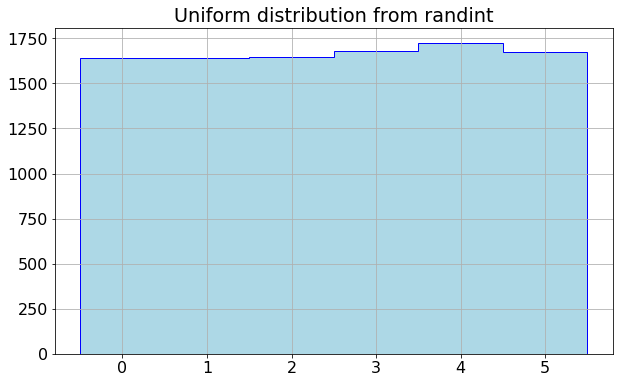
\includegraphics[width=0.7\textwidth]{figures/uniform}
\caption{Uniform distribution generated with \texttt{random.randint} function.}
\label{fig:uniform_dist}
\end{figure}
    
Another module that is capable of generating random numbers is \texttt{numpy}. It has similar functionalities to \texttt{random} but in some cases it fits better to our needs.    
Below an example with \texttt{numpy.random.normal} which allows to throw random numbers according to a normal distribution
(\(\mathcal{N}(0, 1)\)), its plot is shown in Fig.~\ref{fig:gauss_dist}.

\begin{ipython}
from numpy.random import normal
from matplotlib import pyplot as plt

gauss = []
for _ in range(50000):
    gauss.append(normal())

plt.hist(gauss, 100, range=[-4, 4])
plt.title("Example of Gaussian distribution from numpy")
plt.show()
\end{ipython}

\begin{figure}
   \centering
   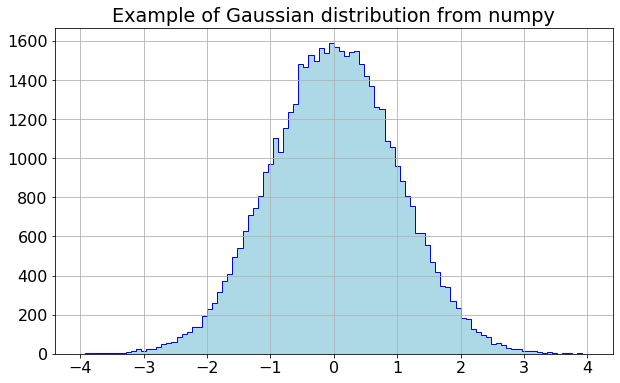
\includegraphics[width=0.7\textwidth]{figures/standard_normal}
   \caption{Normal distribution generated with \texttt{numpy.random.normal} function.}
\label{fig:gauss_dist}
\end{figure}

%\hypertarget{acceptance-rejection-method}{%
%\subsubsection{Acceptance-Rejection
%	Method}\label{acceptance-rejection-method}}
%
%The acceptance-rejection method was proposed by von Neumann in 1951 and
%is used in order to generate random variables that follow a probability
%density function denoted by \(f(x)\). Since we are occasionally
%struggling in inverting the CDF that corresponds to our \(f(x)\), the
%just discussed inverse transform method loses ground and the
%acceptance-rejection method is applied.
%
%Given a so called target distribution \(f(x)\), the acceptance-rejection
%method generates samples according to \(f(x)\) by first of all
%generating samples from a more suitable distribution \(g(y)\).
%Afterwards a random subset of these generated samples is rejected
%according to certain rejection rules. Thereby the choice of this
%rejection rule, or let us call it rejection approach, will be decisive
%if the accepted samples will eventually be distributed according to
%\(f(x)\). The property \(f(x) \leq c\cdot g(x)\), for some constant
%\(c\), tells us now how to generate samples from \(g(y)\). Therefore, we
%conclude that in the acceptance-rejection method a sample \(Y\) is
%generated from \(g\) and at the same time accepted with probability
%\(f(Y)/cg(Y)\). The generic implementation, i.e.~the algorithm of the
%acceptance-rejection method that we can use to sample from density \(f\)
%using candidates from \(g\), can be stated as follows:
%
%\begin{enumerate}
%\def\labelenumi{\arabic{enumi}.}
%\tightlist
%\item
%generate the sample \(Y\) from the distribution with density \(g\)
%\item
%generate \(u\) from \(U[0,1]\), which must be independent of \(Y\)
%\item
%if \(u\leq f(Y)/cg(Y)\), then deliver \(X = Y\), otherwise return to
%step 1.
%\end{enumerate}

\section{Practical Examples of Monte Carlo Simulation}
\label{example-of-monte-carlo-simulation}

In this Section we go through some applications of the Monte Carlo method.

\subsection{Probability to draw two kings from a deck}
Using a frequentist approach, we can calculate the probability of an event as the ratio of the number of favorable outcomes of an experiment (number of successes) and the number of all possible outcomes. 

Imagine we would like to determine the probability of drawing two kings from a standard deck of cards. At the beginning we have 40 cards (i.e. the entire deck) with 4 possible kings, so the probability to get a king is $4/40$. Next, assuming we got a king the first time, we are left with 39 cards and 3 kings only, so the probability to get the second king is $3/39$. Since we want both events to happen, the final probability is the product of the two contributions:

\begin{equation*}
P_\textrm{two kings} = \frac{4}{40} \cdot \frac{3}{39} = \frac{1}{130} \approx 0.0077
\end{equation*}

Let's now try to estimate the same probability with a MC simulation, following the steps outlined above, and check if we get the same number.
\begin{itemize}
\item in this case the domain is a deck of cards. So a list with all the possible cards is defined (with the multiplicative operator (\texttt{*}) a list can be repeated many times; in this case, four times once for each suit). The seed is also set to 1 to make the test reproducible.

\begin{ipython}
from random import sample, choices, seed

seed(1)
deck = ["A", "2", "3", "4", "5", "6", "7", "J", "Q", "K"] * 4
\end{ipython}

\item we draw randomly cards with uniform probability since the deck is fair (all cards have the same probability to be drawn). 
We plan to do 1 million simulations; each time, with the \texttt{sample} function, we pick up two cards from our virtual deck (for debugging purpose the first 10 trials are printed on screen).

\begin{ipython}
trials = 1000000
successes = 0

for i in range(trials):
    cards = sample(deck, k=2)
    if i < 10:
        print (cards)
\end{ipython}

\item at this point we just need to check if the draw is \texttt{['K', 'K']} and in case increase the counter of successes.

\begin{ipython}
    if cards == ["K", "K"]:
        successes += 1
\end{ipython}

\item finally we just print successes/trials which is the sought probability.

\begin{ipython}
print ("The probability to draw two kings is {:.4f}".format(successes/trials))
\end{ipython}
\begin{ioutput}
['Q', '7']
['5', '7']
['J', '2']
['Q', 'A']
['5', '4']
['7', '2']
['2', '5']
['J', 'Q']
['A', 'Q']
['J', '5']

The probability to draw two kings is 0.0077
\end{ioutput}
\end{itemize}
The result is in agreement with our theoretical expectations.

Since we relied on a frequentist approach naively we can say that to get a better accuracy we need to run a larger number of simulations. This becomes apparent playing with the number of trials in the above simulation. 

This is also the main reason why, despite its undoubted power, Monte Carlo simulation is not always the best approach to follow.
Many times indeed the simulation of an experiment requires a lot of computing resources (and time) and it may not be practical to embark into such a large simulation.

\subsection{Determine \(\pi\)}
\label{determine-pi}

Also in this example we know what the result has to look like: \(\pi\approx 3.141592653589793\ldots\) In order to get an estimate through MC simulation of this famous constant a straightforward geometric approach has to be considered. Imagine a circle of diameter \(D\) which is inscribed in a square with side length \(D\), see Fig.~\ref{fig:circle_inscribed}.

\begin{figure}[htb]
	\centering
	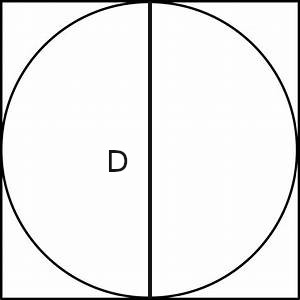
\includegraphics[width=0.3\textwidth]{figures/circle_inscribed.jpeg}
	\caption{A circle of diameter $D$ inscribed in a square.}
	\label{fig:circle_inscribed}
\end{figure}

Computing the ratio of the area of the two figures

\begin{equation}
\frac{\textrm{Area Circle}}{\textrm{Area Square}} = \frac{\pi D^2/4}{D^2} = \frac{\pi}{4} 
\end{equation}

The algorithm to approximate \(\pi\) should then be

\begin{itemize}
\item select 2 random numbers, \(x_1\) and \(x_2\), from the interval
\([0,D]\); 
\item determine if the point defined by the ordered pair
\((x_1, x_2)\) lies within or on the circle, keeping track both of the total number of tested points and of those satisfying the condition \(D \le\sqrt{x_1^2 + x_2^2}\); 
\item approximate the ratio of the areas by the number of points within or on the circle divided by the total number of tested points; 
\item multiply the approximated area by 4 to get \(\pi\).
\end{itemize}

\begin{ipython}
from random import random, seed
from math import sqrt

seed(1)
in_circle = 0.0
trials = 100000
for _ in range(trials):
    x1 = random()
    x2 = random()
    r = sqrt(pow(x1, 2) + pow(x2, 2))
    if r <= 1:
        in_circle += 1

print ("Approx. pi: {}".format(in_circle/trials*4))
\end{ipython}
\begin{ioutput}
Approx. pi: 3.13944
\end{ioutput}

The lower is the probability we try to estimate with MC the higher has to be the number of simulations. 
The result precision indeed depends on the number of "successes" and if the success probability is small, many trials are needed. This can be simply checked by playing with the number of simulations in the previous examples. For example we may run an entire set without getting two consecutive kings, nevertheless we cannot conclude there is zero probability of such event.

The only conclusion we can draw is that Monte Carlo simulation is not always the best approach to follow, especially for computationally heavy experiments.

In the following example it is apparent how changing the number of simulations in a single experiment the approximation precision improves. In Fig.~\ref{fig:circle_approx} it is shown graphically the results with 100, 1000, 10000, 100000 and 1000000 simulations.

\begin{ipython}
from random import random, seed
from math import sqrt
import numpy as np

seed(1)
trials=[100, 1000, 10000, 100000, 1000000]
for i, t in enumerate(trials):
    in_circle = 0
    circ = []
    squa = []
    for _ in range(t):
        x1 = random()-0.5
        x2 = random()-0.5
        r = sqrt(pow(x1, 2)+pow(x2, 2))

        if r <= 0.5:
            in_circle += 1
            circ.append((x1, x2))
        else:
            squa.append((x1, x2))
    print (in_circle/t*4)
\end{ipython}
\begin{ioutput}
3.12
3.096
3.1212
3.13956
3.142136
\end{ioutput}

\begin{figure}[htb]
\centering
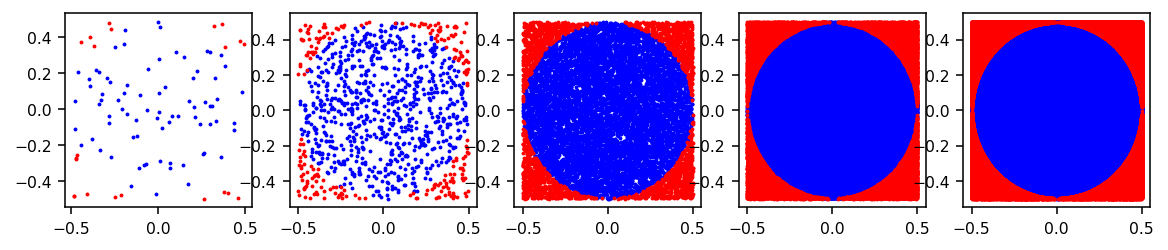
\includegraphics[width=0.7\textwidth]{figures/mc_vs_n_experiments}
\caption{Graphical representation of geometrical approximation of $\pi$. Results are reported for $N = 100, 1000, 10000, 100000, 1000000$ simulations. It is clear how the result improves with $N$.}
\label{fig:circle_approx}
\end{figure}

\section{Accuracy of Monte Carlo Simulation}
\label{sec:confidence_interval}

* Assume you don't know the probability of getting to K from two consecutive draws
    * what can be concluded from the result of a single MC experiment ?
    
   \begin{ipython}
# define the domain of inputs
from random import sample, seed

deck = ['A', 'K', 'J', 'Q', '7', '6', '5', '4', '3', '2'] * 4

seed(97)
def deck_sim(trials):
    successes = 0.0
    for _ in range(trials):
        cards = sample(deck, 2)
        if cards == ['K', 'K']:
            successes += 1
    return successes

trials = 10000
successes = deck_sim(trials)
print (successes/trials)
   \end{ipython}
\begin{ioutput}
0.0084
\end{ioutput}

The central limit  theorem~\cite{bib:central_limit} states that if we have \(Y_1, Y_2,\dots, Y_n\) which are random samples from a distribution \(Y\) with true mean \(\mu\) and variance \(\sigma^{2}\), then with \(n\) sufficiently large,

\begin{equation*} 
\mu_n = \cfrac{1}{n}\sum_i^n Y_i
\end{equation*}
has approximately a normal distribution \(\mathcal{N}(\mu, \sigma^2/n)\).

This means that if one repeats the MC experiment many times (changing the seed of the random number generator) would obtain results normally distributed around the \emph{true} value \(\mu\).
We can check the central limit theorem by repeating many times the MC experiment with our virtual deck and check how the distribution of $\mu_n$ behaves.

\begin{ipython}
# define the domain of inputs
import numpy as np
from random import sample, seed

deck = ['A', 'K', 'Q', 'J', '2', '3', '4', '5', '6', '7'] * 4
experiments = 1000
trials = 10000
r = []

seed(1)
for e in range(experiments):
    successes = 0.0
    for i in range(trials):
        cards = sample(deck, 2)
        if cards == ['K', 'K']:
            successes += 1
    r.append(successes/trials)

print ("Mean: {:.6f}".format(np.mean(r)))
print ("Std : {:.6f}".format(np.std(r)))
\end{ipython}
\begin{ioutput}
Mean:  0.007688
Std :  0.000871
\end{ioutput}

Looking at Fig.~\ref{fig:repeated_MC} it is clear that the various results are distributed as a Gaussian.

\begin{figure}[htb]
\centering
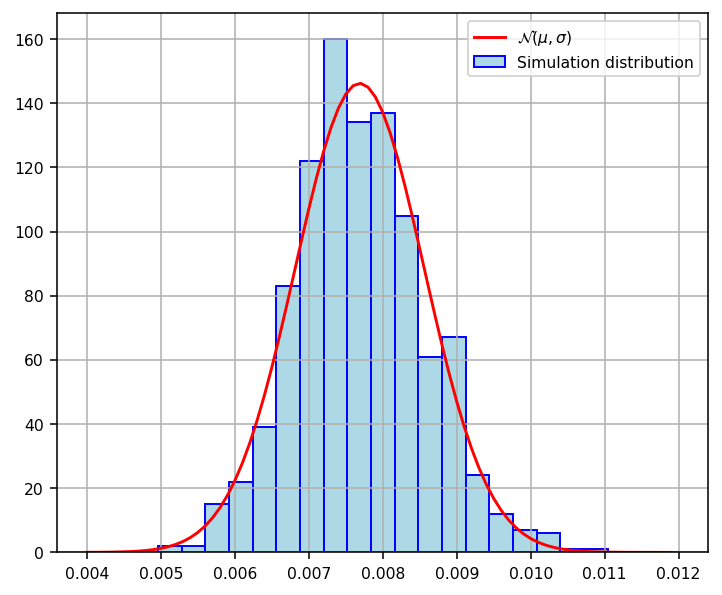
\includegraphics[width=1\textwidth]{figures/experiment_distribution}
\caption{Distribution of the results of 1000 experiments.}
\label{fig:repeated_MC}
\end{figure}

From the central limit theorem hence: 

\begin{equation}
\mu_n - \mu \approx \mathcal{N}(0, \sigma^2/n)
\end{equation}

From the previous equation and remembering the definition of  quantiles~\ref{sec:quantile-function} it is possible to define an interval so that there is a certain probability to find $\mu$ in there. Referring to Fig.~\ref{fig:confidence_interval} we can write:

\begin{equation}
P\left(\mu_n - \cfrac{1.96\sigma}{\sqrt{n}}\le \mu \le \mu_n + \cfrac{1.96\sigma}{\sqrt{n}}\right) = 0.95
\end{equation}
probability which correspond to the shaded pink area.

\begin{figure}[htb]
	\centering
	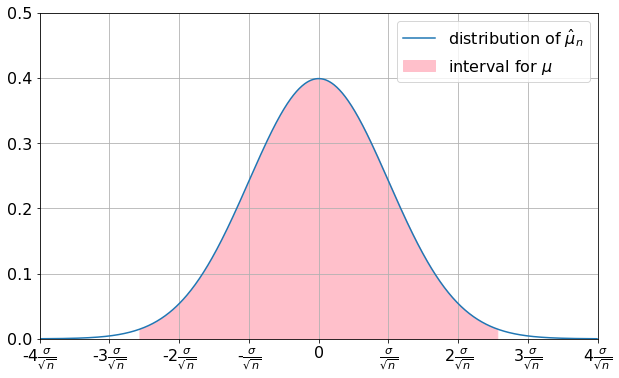
\includegraphics[width=0.7\textwidth]{figures/confidence_interval}
	\caption{Confidence interval for a MC experiment.}
	\label{fig:confidence_interval}
\end{figure}

This interval is called \textbf{95\% confidence interval} because it covers 95\% of the total area under the Gaussian. It can be interpreted like the following: if you repeat many times a simulation, the fraction of calculated confidence intervals that contains the true parameter $\mu$ would tend toward 95\%.

The most commonly used intervals are 99\% and 95\% confidence level and are respectively defined as \(\pm \cfrac{2.57\sigma}{\sqrt{n}}\) and \(\pm \cfrac{1.96\sigma}{\sqrt{n}}\).

To construct an interval with a custom confidence level $\alpha$, we have to find a number $A$ such that
\begin{equation}
\Phi(A) = 1 - \frac{1-\alpha}{2}\quad\implies\quad A = \Phi^{-1}\left(\cfrac{1+\alpha}{2}\right)
\label{for:A}
\end{equation}
then the $\alpha$-confidence interval guarantees
\begin{equation}
P(\mu - A\sigma \le X \le \mu+ A\sigma) = \alpha 
\end{equation}

Below an example of how to compute a confidence level in \texttt{python} given a set of fake simulations. Note that the inverse of the Gaussian CDF ($\Phi^{-1}$), used in Equation~\ref{for:A}, is computed with the method \texttt{norm.ppf()} (more details on CDF in Section~\ref{sec:quantile-function}).

\begin{ipython}
import numpy as np
from scipy.stats import norm

samples = [1.,2.,3.,4.,4.,4.,5.,5.,5.,5.,4.,4.,4.,6.,7.,8.]
alpha = 0.95
X = np.array(samples)
A = norm.ppf((1 + alpha)/2)
m, se = np.mean(X), np.std(X)
h = A*se/np.sqrt(len(samples))
print ("{:.0f}% confidence int.: {:.3f} +- {:.3f}".format(alpha*100, m, h))
\end{ipython}
\begin{ioutput}
95% confidence int.: 4.437 +- 0.812
\end{ioutput}

The confidence interval can be used to assess the accuracy of a Monte Carlo simulation. From what has been said above the uncertainty on our best estimate of $\mu$ is $\sqrt{\cfrac{\sigma^2}{n}}=\cfrac{\sigma}{\sqrt{n}}$ where \(\sigma^2 = \mathrm{Var}(Y)\).

While it is obvious that the estimate should get worse with increased variance and better with increased sample size, this equation  gives us the exact scaling. Indeed the uncertainty formula tells us that to get one more decimal digit of accuracy (i.e. an error one tenth as large) requires a 100-fold increase in computation. To get three more digits of accuracy requires one million times as much computation. From that it is clear that Monte Carlo computation is poorly suited for problems that must be answered with high precision.

\section*{Exercises}
\begin{question}
Using the function \texttt{randint} of the module \texttt{random} make a Monte Carlo simulation of rolling three dices to check the probability of getting the same values on the three of them.
From the probability theory you should expect:

\[P_{d1=d2=d3} = \frac{1}{6}\cdot\frac{1}{6}\cdot\frac{1}{6}\cdot 6 = \frac{1}{36} = 0.0278\]
\end{question}

\cprotEnv\begin{solution}
\begin{ipython}
from random import seed, randint

seed(1)
trials = 10000000
success = 0

for _ in range(trials):
    d1, d2, d3 = randint(1, 6), randint(1, 6), randint(1, 6)
    if d1 == d2 and d2 == d3:
        success += 1

print ("The probability to get three equal dice is {:.4f}".format(success/trials))

The probability to get three equal dice is 0.0278
\end{ipython}
\end{solution}

\begin{question}
Two fair dice are rolled, find the probability that their sum is:
\begin{enumerate}[start=1]
	\item equal to 1;
	\item equal to 4;
	\item less than 13.
\end{enumerate}
	
\noindent\textbf{Hint:} the possible combinations of the outcomes of two dice are 36 (to realize it you can simply think that for each one of the six faces of the first die you have six possible faces of the second hence $6\cdot 6=36$). It is not possible to get 1 since the dice have no face with 0 so the first probability should come out 0. The sum of the two dice is always less than 13 (the maximum is 12\ldots) so the answer to point 3 is 1. We can get a sum of 4 in 3 cases (1-3, 3-1 or 2-2) so the expected probability is $3/36=1/12=0.0833$
\end{question}

\cprotEnv\begin{solution}
\begin{ipython}
import random

random.seed(1)
successes = {"=1":0.0, "=4":0.0, "<13":0.0}
trials = 100000

for _ in range(trials):
    d1 = random.randint(1, 6)
    d2 = random.randint(1, 6)

    if (d1 + d2) == 1:
        successes["=0"] += 1.0
    if (d1 + d2) == 4:
        successes["=4"] += 1.0
    if (d1 + d2) < 13:
        successes["<13"] += 1.0

for k,v in successes.items():
    print ("P({}): {:.3f}".format(k, v/trials))

P(=1): 0.000
P(=4): 0.084
P(<13): 1.000
\end{ipython}
\end{solution}

\begin{question}
There are 60 chemical flasks in the laboratory, 6 of which are incorrectly labeled. What is the chance that if we randomly choose 5 flasks, exactly 3 of them will be labeled correctly ?

\noindent\textbf{Hint:} the probability is approximately 0.5 \%.
\end{question}

\cprotEnv\begin{solution}
\begin{ipython}
import random

flasks = ["C"]*54 + ["U"] * 6
random.seed(1)
trials = 1000
success = 0.

for _ in range(trials):
    draw = random.sample(flasks, 5)
    if draw.count("U") == 3:
        success += 1.

print ("Probability: {:.3f}%".format(success/float(trials)*100))

Probability: 0.499%
\end{ipython}
\end{solution}

\begin{question}
Given the following historical series (1895-2020) find average September temperature in US and report the 99\% confidence interval of your measure.
\noindent
Input (temperatures are in Fahrenheit degrees): \href{https://raw.githubusercontent.com/matteosan1/finance_course/develop/libro/input_files/histo_temp.csv}{histo\_temp.csv}
\end{question}

\cprotEnv\begin{solution}
\begin{ipython}
from scipy.stats import norm
import numpy as np
import pandas as pd

# first download the input file
df = pd.read.csv("histo_temp.csv")
temperatures = df['T'].to_array()
alpha = 0.99

A = norm.ppf((1 + alpha)/2)
m, se = np.mean(temperatures), np.std(temperatures)
h = A*se/np.sqrt(len(temperatures))

print ("Avg temperature in September (US): {:.1f}".format(m))
print ("{:.1f}% confidence interval: +- {}".format(alpha*100, h))
Avg temperature in September (US): 65.1
99% confidence interval: +- 0.3
\end{ipython}
\end{solution}

\begin{question}
Using the function \texttt{normal} of \texttt{numpy.random} simulate the price of a stock which evolves according to a log-normal stochastic process with a daily rate of return \(\mu=0.1\) and a volatility \(\sigma=0.15\) for 30 days.
Also plot the price. Try to play with \(\mu\) and \(\sigma\) to see how the plot changes.
\end{question}

\cprotEnv\begin{solution}
\begin{ipython}
from numpy.random import normal, seed
from matplotlib import pyplot as plt
import math

S = 100
mu = 0.1
sigma = 0.15
T = 1
seed(1)

historical_series = [S]
for i in range(30):
    S = S * math.exp((mu - 0.5 * sigma * sigma) * T +
        sigma * math.sqrt(T) * normal())
    historical_series.append(S)

plt.plot(range(31), historical_series)
plt.xlabel("days")
plt.ylabel("Price of stock X")
plt.show()
\end{ipython}

\begin{figure}[htbp]
\begin{center}
  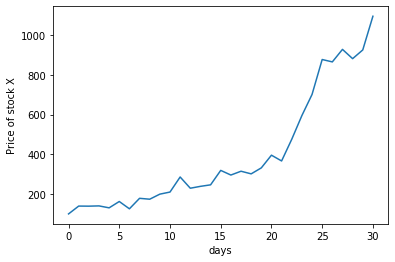
\includegraphics[width=0.7\linewidth]{figures/lesson6_solutions_5_0.png}
\end{center}
\end{figure}
\end{solution}


\begin{thebibliography}{9}
\bibitem{bib:monte_carlo}\href{https://www.youtube.com/watch?v=OgO1gpXSUzU}{\emph{Monte Carlo Simulation}}, MIT Course [Online]
\bibitem{bib:central_limit} \href{https://en.wikipedia.org/wiki/Central_limit_theorem}{\emph{Central Limit Theorem}}, Wikipedia [Online]
\bibitem{bib:confidence_interval}\href{https://www.statisticshowto.com/probability-and-statistics/confidence-interval}{\emph{Confidence Interval: How to Find a Confidence Interval: The Easy Way!}}, Statistic Howto [Online]
\end{thebibliography}









